\setcounter{paragraph}{0}
\PhanI
\begin{ex}
Một con lắc đồng hồ đang dao động tắt dần, mỗi chu kì năng lượng bị mất đi do ma sát là $0,01\ J$. Để duy trì dao động của con lắc đồng hồ, ta cần cung cấp cho con lắc một năng lượng
\choice
{lớn hơn $0,01\ J$ trong mỗi chu kì}
{lớn hơn $0,01\ J$ trong mỗi nửa chu kì}
{\True vừa bằng $0,01\ J$ trong mỗi chu kì}
{lớn hơn $0,01\ J$ trong mỗi nửa chu kì}
\loigiai{}
\end{ex}
%\loai{Dao động cưỡng bức}
\begin{ex}
Một vật dao động điều hòa với tần số riêng $f_0 = 5\ Hz$. Ngoài dao động riêng, vật còn chịu tác dụng của ngoại lực cưỡng bức tuần hoàn có tần số $f = 7,5\ Hz$. Sau khi vật đạt trạng thái dao động ổn định, tần số dao động của hệ là
\choice
{$12,5\ Hz$}
{\True $7,5\ Hz$}
{$5\ Hz$}
{$2,5\ Hz$}
\loigiai{}
\end{ex}
\begin{ex}%[3P1-19.2B][Loai1]
Một con lắc lò xo gồm lò xo nhẹ có độ cứng $100\ N/m$ gắn với một vật nhỏ có khối lượng 1 kg. Tác dụng một ngoại lực $F_n=F_0\cos \left({10\pi t-2,017}\right)$ N để con lắc dao động cưỡng bức. Khi đó vật dao động nhỏ với tần số là
\choice
{$\dfrac{5}{\pi }$ Hz}
{\True 5 Hz}
{10 Hz}
{$\dfrac{1}{5}$ Hz}
\loigiai{
Dao động cưỡng bức có tần số bằng với tần số của ngoại lực cưỡng bức $f=5\ Hz$. }
%\haidong{4}
\end{ex} \haidong{20}
\begin{ex}%[3P1-19.1K][Loai1]
Một vật dao động cưỡng bức do tác dụng của ngoại lực $F = 0,5\cos 10\pi t$ (F tính bằng N, t tính bằng s). Vật dao động cưỡng bức với
\choice
{tần số góc 10 rad/s}
{chu kì 2 s}
{biên độ 0,5 m}
{\True tần số 5 Hz}
\loigiai{
Giai đoạn ổn định: $f_0=f=\dfrac{\omega}{2\pi}=5\ Hz$.
}
%\haidong{4}
\end{ex} \haidong{20}

\begin{ex}%[3P1-19.2K][Loai1]
Một con lắc đơn gồm vật có khối lượng m, dây treo có chiều dài 2 m. Lấy $g=\pi^2$. Con lắc dao động điều hòa dưới tác dụng của ngoại lực có biểu thức $F = F_0\cos \left(\omega t + 0,5\pi\right)$ N. Nếu chu kì T của ngoại lực tăng từ 2 s lên 4 s thì biên độ dao động của vật sẽ
\choice
{\True tăng rồi giảm}
{giảm rồi tăng}
{chỉ giảm}
{chỉ tăng}
\loigiai{
\begin{itemize}
\item Chu kì dao động riêng của vật: $T_0=\dfrac{2\pi}{\omega}=\dfrac{2\pi}{\sqrt{\dfrac{g}{\ell}}}=2\sqrt{2}\ s $.
\item Nếu chu kì T của ngoại lực tăng từ 2 s lên 4 s thì biên độ dao động của vật sẽ tăng rồi giảm  (Cực đại khi $T =  2\sqrt{2}\ s $ : Cộng hưởng).
\end{itemize}
}
%\haidong{4}
\end{ex} \haidong{20}
\begin{ex}%[3P1-19.2K][Loai1]
Một con lắc lò xo gồm vật nhỏ khối lượng 50 g, lò xo có độ cứng 50 N/m, dao động trên mặt phẳng ngang có ma sát. Lấy gần đúng ${\pi^2} = 10$. Tác dụng vào con lắc một lực biến thiên điều hoà theo thời gian, giữ nguyên biên độ ngoại lực tăng dần tần số lực tác dụng vào con lắc từ 3 Hz đến 7 Hz. Điều nào sau đây mô tả đúng dao động của con lắc?
\choice
{\True Biên độ dao động cưỡng bức tăng dần đến cực đại rồi giảm xuống}
{Biên độ dao động cưỡng bức tăng dần}
{Con lắc dao động cưỡng bức với biên độ tăng dần, tần số không đổi}
{Biên độ dao động cưỡng bức không đổi trong suốt thời gian khảo sát}
\loigiai{
\begin{itemize}
\item Tần số dao động riêng của vật $f_0=\dfrac{\omega}{2\pi}=\dfrac{\sqrt{\dfrac{k}{m}}}{2\pi}=5\ Hz$.
\item Giữ nguyên biên độ ngoại lực tăng dần tần số lực tác dụng vào con lắc từ 3 Hz đến 7 Hz thì biên độ dao động cưỡng bức tăng dần đến cực đại rồi giảm xuống. (Cực đại khi $f = 5$ Hz: Cộng hưởng).
\end{itemize}
}
%\haidong{4}
\end{ex} \haidong{20}
\begin{ex}%[3P1-19.2K][Loai1]
Một con lắc lò xo gồm vật nặng 100 g và lò xo có độ cứng 40 N/m. Tác dụng lên vật một ngoại lực biến đổi tuần hoàn theo thời gian có biên độ $F_0$ và tần số $f_1= 4$ Hz thì biên độ dao động vật trong giai đoạn ổn định là $A_1$. Nếu giữ nguyên biên độ $F_0$ và tăng tần số ngoại lực lên $f_2 = 4,5$ Hz thì biên độ dao động vật trong giai đoạn ổn định là $A_2$. So sánh $A_1$ và $A_2$?
\choice
{$A_1\ge A_2$}
{$A_1<A_2$}
{$A_1=A_2$}
{\True $A_1>A_2$}
\loigiai{
\begin{itemize}
\item Tần số dao động riêng của vật $f_0=\dfrac{\omega}{2\pi}=\dfrac{\sqrt{\dfrac{k}{m}}}{2\pi}=3,2\ Hz$.
\item Biên độ dao động của hệ phụ thuộc vào độ chênh lệch giữa tần số dao động riêng của vật $f_0$ và tần số f dao động của ngoại lực (hay $\left|f - f_0\right|$).
\item Khi tần số của lực cưỡng bức càng gần tần số dao động riêng thì biên độ dao động cưỡng bức càng lớn. 
\item Ta có $\left|f_1-f_0\right|<\left|f_2-f_0\right|\Rightarrow A_1>A_2$.
\end{itemize}
}
%\haidong{5}
\end{ex} \haidong{20}

\begin{ex}%[3P1-19.2K][Loai1]
Một con lắc lò xo gồm vật khối lượng $m = 100$  g, lò xo có độ cứng $k = 100$ N/m.  Cho $\pi^2 = 10$.  Trong cùng một điều kiện về lực cản của môi trường thì biểu thức ngoại lực điều hoà nào sau đây làm cho con lắc dao động cưỡng bức với biên độ lớn nhất?
\choice
{$F = F_0\cos (2\pi t + \pi )$ N}
{$F = F_0\cos (20\pi t + \dfrac{\pi}{2})$ N}
{\True $F = F_0\cos (10\pi t)$ N}
{$F = F_0\cos (8\pi t)$ N}
\loigiai{
Con lắc dao động cưỡng bức với biên độ lớn nhất $ \Leftrightarrow \omega =\omega_0=\sqrt{\dfrac{k}{m}}=10\pi \ rad/s. $ (Cộng hưởng)
$\Rightarrow$ $F = F_0\cos \left(10\pi t\right)$  N}
%\haidong{4}
\end{ex} \haidong{20}

%\loai{Cộng hưởng}
\begin{ex}
\immini[thm]{
Các cơ vận động nhãn cầu tạo ra chuyển động của nhãn cầu và chuyển động đồng bộ của mi mắt. Các cơ giữ nhãn cầu này co giãn và có thể coi gần đúng như những lò xo có độ cứng tương đương là k. Các nghiên cứu y khoa cho thấy, nếu đầu người bị rung lắc với tần số 29 Hz thì thị lực sẽ mờ đi do tần số rung lắc này cộng hưởng với tần số dao động riêng của nhãn cầu. Nếu khối lượng trung bình của một nhãn cầu người bình thường là 7,5 g thì độ cứng tương đương của hệ thống cơ giữ nhãn cầu là
\choice
{$0,226\ N/m$}
{$0,113\ N/m$}
{$0,452\ N/m$}
{$0,891\ N/m$}
}{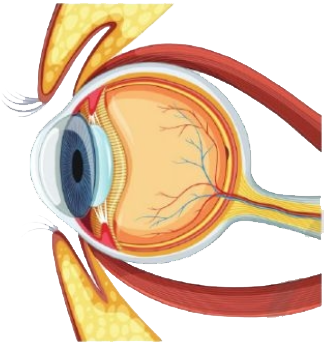
\includegraphics[width=4cm]{Hinh/CDH5}}
\loigiai{
Hiện tượng cộng hưởng: $f=f_0\Rightarrow \dfrac{1}{2\pi}\sqrt{\dfrac{k}{m}}=f_0\Rightarrow k\approx 0,226\ N/m$.
}
%\haidong{4}
\end{ex} \haidong{20}
\begin{ex}
Một người chở hai thùng nước ở phía sau xe đạp và đạp xe trên con đường lát bê tông. Cứ cách 3 m, trên đường lại có một rãnh nhỏ. Biết chu kì dao động riêng của nước trong thùng là 0,6 s. Đối với người đó tốc độ nào sau đây bất  lợi nhất? 
\choice
{\True 5 m/s}
{6 m/s}
{13 m/s}
{14 m/s}
\loigiai{

}
%\haidong{5}
\end{ex} \haidong{20}


\begin{ex}%[3P1-19.2K][Loai1] 
Một con lắc lò xo gồm lò xo có độ cứng $100\ N/m$ và vật nhỏ có khối lượng m. Tác dụng lên vật ngoại lực $F=20\cos10\pi t$ N (t tính bằng s) dọc theo trục lò xo thì xảy ra hiện tượng cộng hưởng. Lấy $\pi ^2= 10$. Giá trị của m là
\choice
{$0,4\ kg$}
{$1\ kg$}
{$250\ g$}
{\True $100\ g$}
\loigiai{
\begin{itemize}
\item Từ phương trình ngoại lực, ta có: $\omega _F=10\pi\ rad/s$.
\item Để xảy ra cộng hưởng thì tần số dao động riêng của hệ phải bằng với tần số dao động của ngoại lực: $\omega _F=\sqrt{\dfrac{k}{m}}\Leftrightarrow 10\pi =\sqrt{\dfrac{100}{m}}\Rightarrow m=0,1\ kg=100\ g$.
\end{itemize}}
%\haidong{5}
\end{ex} \haidong{20}


\begin{ex}
Một con lắc lò xo dao động tắt dần theo phương ngang với chu kì $T = 0,2\  s$. Vật nhỏ dao động có khối lượng $100\ g$. Hệ số ma sát giữa vật và mặt phẳng ngang là $0,01$. Độ giảm biên độ của vật sau một nửa chu kì dao động là
\choice
{0,4 cm}
{0,3 cm}
{\True 0,2 cm}
{0,2 m}
\loigiai{}
\end{ex}
\begin{ex}
Một con lắc lò xo dao động điều hòa với chu kì $T = \dfrac{\pi}{10}\ s$, một đầu cố định, đầu còn lại gắn vật nặng khối lượng $m = 0,25\ kg$. Con lắc dao động cuỡng bức theo phương trùng với trục của lò xo dưới tác dụng của ngoại lực tuần hoàn $F = F_{0} \cdot \cos (\omega t)$ (N). Thay đổi tần số góc $\omega$ từ giá trị $10\ rad/s$ đến $15\ rad/s$ thì biên độ dao động
\choice
{\True tăng lên}
{tăng lên rồi giảm xuống}
{không thay đổi}
{giảm xuống rồi tăng lên}
\loigiai{}
\end{ex}
\begin{ex}
Một vật dao động điều hòa có phương trình $x = 2 \cos (10 t)\ cm$. Bỏ qua lực cản của môi trường. Lần lượt tác dụng lên vật các ngoại lực cượng bức $F_{1} = 10\cos \left(6t + \dfrac{\pi}{3}\right)\ N$; $F_{2} = 10\cos \left(8 t + \dfrac{2 \pi}{3}\right)\ N$ và $F_{3} = 10\cos \left(18t - \dfrac{2 \pi}{3}\right)\ N$. Biên độ dao động cưỡng bức của vật
trong ba trường hợp có biên độ lần lượt là $A_{1}$; $A_{2}$ và $A_{3}$. Khi dao động đến giai đoạn ổn định. Phát biểu nào sau đây là đúng?
\choice
{$A_{1} = A_{2} > A_{3}$}
{$A_{1} = A_{3} > A_{2}$}
{$A_{1} = A_{2} = A_{3}$}
{\True $A_{3} < A_{1} < A_{2}$}
\loigiai{}
\end{ex}
\begin{ex}%[3P1-20.1K][Loai1]
Một con lắc dao động tắt dần. Sau một chu kì biên độ giảm 12\%. Phần năng lượng mà con lắc đã mất đi trong một chu kì
\choice
{24\%}
{12\%}
{88\%}
{\True 22,56\%}
\loigiai{
\begin{itemize}
\item Biên độ còn lại sau mỗi chu kì: $A_1=0,88A$.
\item Phần năng lượng đã mất đi sau mỗi chu kì: $\dfrac{\Delta W}{W} = 1 - \dfrac{0,88^2.A^2}{A^2} = 0,2256 = 22,56\%$. 
\end{itemize}
}
%\haidong{5}
\end{ex} \haidong{20}
\begin{ex}
Một vật dao động tắt dần, sau 8 chu kì dao động liên tiếp thì cơ năng của vật giảm $48 \%$ so với cơ năng ban đầu. Sau mỗi chu kì dao động, biên độ dao động giảm xấp xỉ
\choice
{1 \%}
{2 \%}
{3 \%}
{\True 4 \%}
\loigiai{}
\end{ex}
%\loai{Quãng đường vật đi được cho đến khi dừng lại}
\begin{ex}%[3P1-20.1G][Loai1]
Một con lắc lò xo gồm một vật nhỏ có khối lượng 0,5 kg và lò xo có độ cứng $k=80\ N/m.$ Vật nhỏ được đặt trên giá đỡ cố định nằm ngang trục lò xo. Hệ số ma sát giữa vật và giá đỡ là 0,02. Ban đầu giữ vật ở vị trí lò xo nén 5,25 cm rồi buông nhẹ để con lắc lò xo dao động tắt dần. Lấy $g=10\ m/s^2$. Quãng đường tổng cộng vật đi được từ lúc dao động đến khi dừng hẳn là
\choice
{\True $1,1025\ m$}
{$2,25\ m$}
{$1,25\ m$}
{$2,5\ m$}
\loigiai{
\begin{itemize}
\item Gọi $\Delta A_{\frac{1}{2}}$ là độ giảm biên độ sau nửa chu kì.
\item Ta có: $x_0=\dfrac{F_c}{k}=\dfrac{{\mu mg}}{k}=\dfrac{0,02.0,5.10}{80}=1,25.10^{-3}\ m$.
\item Xét: $\dfrac{A}{\Delta A_{\frac{1}{2}}}=\dfrac{A}{2x_0}=\dfrac{0,0525}{2.1,25.10^{-3}}=21$.
\item Vì $q=0$ nên vật dừng lại ở vị trí bằng: $S=\dfrac{A^2}{\Delta A_{\frac{1}{2}}}=\dfrac{A^2}{2x_0}=\dfrac{{0,0525^2}}{2.1,25.10^{-3}}=1,1025\ m$.
\end{itemize}}
%\haidong{10}
\end{ex} \haidong{20}

\begin{ex}%[3P1-20.1K][Loai1]
Một con lắc lò xo đang dao động tắt dần. Người ta đo được độ giảm tương đối của biên độ trong 3 chu kì đầu tiên là 10\%. Độ giảm tương đối của cơ năng tương ứng \textbf{gần nhất} với giá trị nào sau đây?
\choice
{9\%}
{\True 19\%}
{3\%}
{25\%}
\loigiai{
\begin{itemize}
\item Theo đề bài: $\dfrac{\Delta A}{A_0} = 10\%$ $\Rightarrow \Delta A = 0,1A_0 \Rightarrow A_1 = A_0 - 0,1A_0 = 0,9A_0$.
\item Độ giảm tương đối của cơ năng được xác định bằng $\dfrac{\Delta W}{W}$.
\item Ta có: $\dfrac{\Delta W}{W} = \dfrac{\dfrac{1}{2}kA_0^2 - \dfrac{1}{2}kA_1^2}{\dfrac{1}{2}kA_0^2} = \dfrac{A_0^2 - A_1^2}{A_0^2} = \dfrac{A_0^2 - (0,9A_0)^2}{A_0^2} = 0,19=19$\%.
\end{itemize}
}
%\haidong{7}
\end{ex} \haidong{20}
\PhanII
\setcounter{ex}{0}
\begin{ex}
\immini[thm]{Máy đo địa chấn được sử dụng để phát hiện và đo đạc những rung động địa chấn được tạo ra bởi sự dịch chuyển của lớp vỏ Trái Đất. Tần số của những cơn địa chấn thường nằm trong khoảng $30\ Hz - 40\ Hz$. Năng lượng từ các cơn địa chấn có khả năng kích thích con lắc lò xo bên trong máy đo làm đầu bút di chuyển để vẽ lên giấy như hình.}{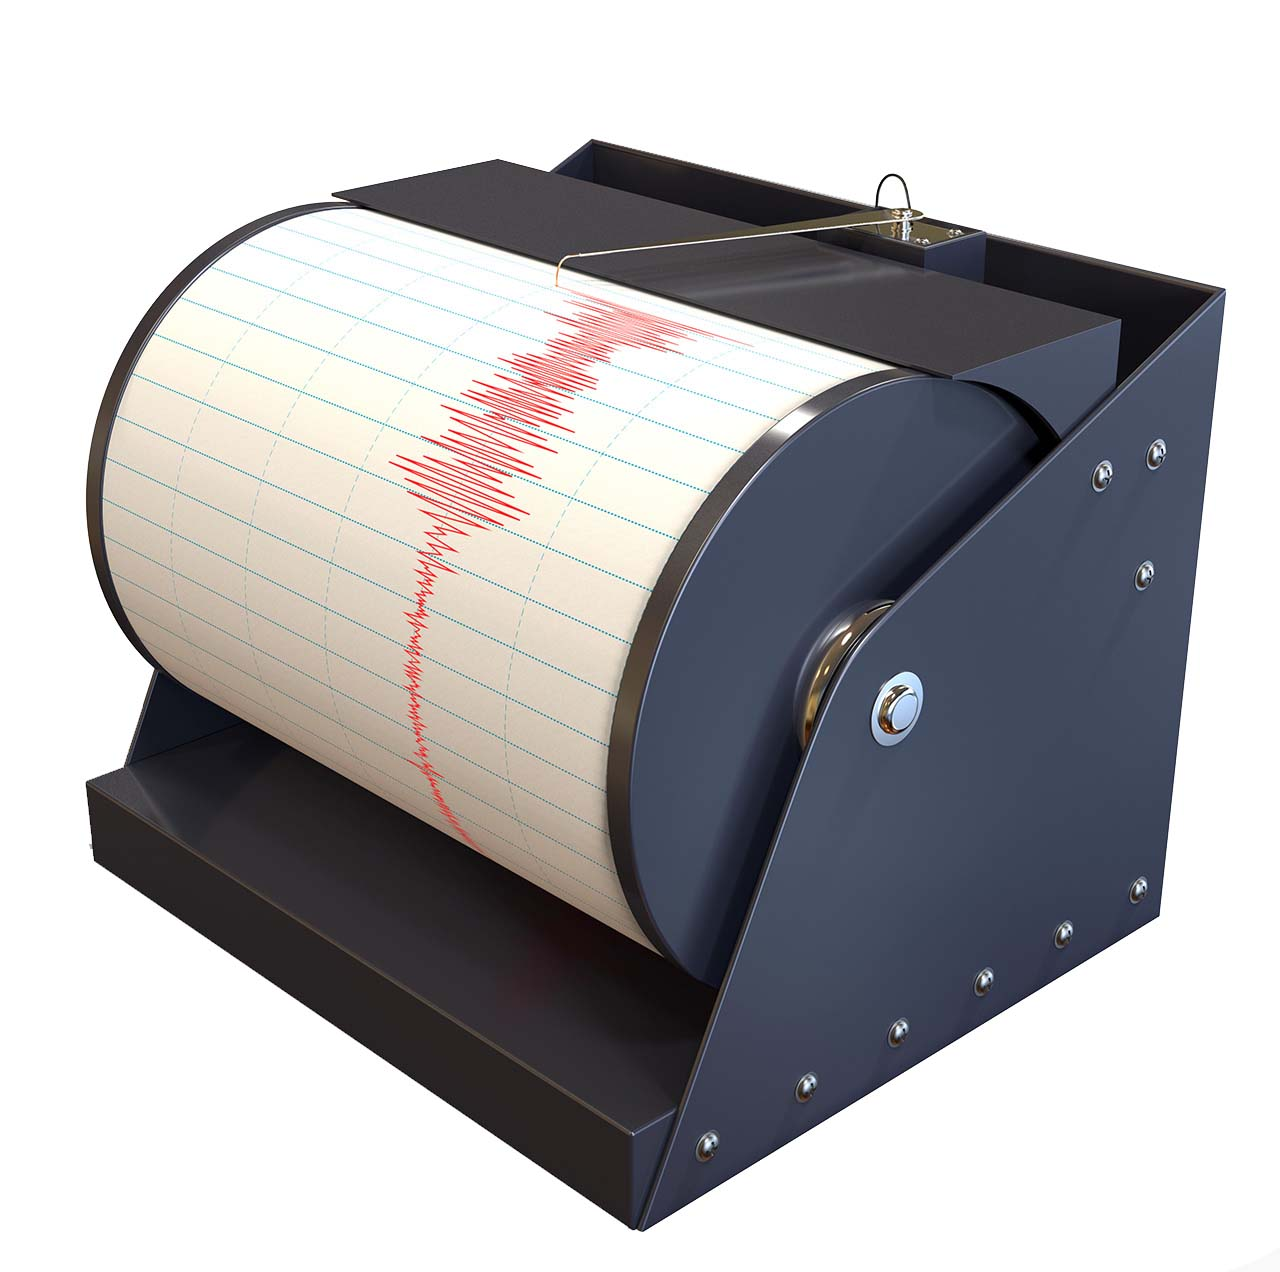
\includegraphics[width=3cm]{Images/31965}}
\choiceTF[t]
{Dao động của con lắc lò xo trong máy đo địa chấn là dao động duy trì}
{Đầu bút di chuyển và vẽ được lên tờ giấy là do các cơn địa chấn tạo ra dao động duy trì}
{\True Tần số dao động của những con lắc lò xo trong máy địa chấn vào khoảng $30\ Hz - 40\ Hz$}
{Để máy địa chấn ghi nhận được kết quả tốt nhất thì tần số riêng của con lắc lò xo phải có giá trị thật lớn hơn $40\ Hz$}
\loigiai{
\begin{itemchoice}
\itemch 
\itemch 
\itemch 
\itemch 
\end{itemchoice}
}
\end{ex}
\begin{ex}
Cho các nhận định sau về một con lắc dao động tắt dần.
\choiceTF[t]
{\True Cứ sau mỗi chu kì năng lượng giảm đi $8 \%$. Phần trăm biên độ dao động mất đi trong một dao động toàn phần xấp xỉ 4\%}
{Cứ sau mỗi chu kì biên độ giảm đi $3 \%$. Phần năng lượng của con lắc bị mất đi trong một dao động toàn phần xấp xỉ $9 \%$}
{Cứ sau mỗi chu kì, năng lượng của con lắc giảm $5 \%$. Sau 2 chu kì dao động liên tiếp biên độ giảm  xấp xỉ  $5 \%$}
{Nếu cơ năng ban đầu của nó là $8 \ J$. Sau ba chu kì đầu tiên biên độ của nó giảm đi $10 \%$. Phần năng lượng chuyển thành nhiệt sau khoảng thời gian đó  xấp xỉ  $2,7 \ J$}
\loigiai{
\begin{itemchoice}
\itemch
\itemch
\itemch
\itemch
\end{itemchoice}
}
%\haidong{8}
\end{ex} \haidong{20}
\begin{ex}
Con lắc lò xo có độ cứng $64\ N/m$ một đầu cố định, đầu còn lại gắn vật có khối lượng m dao động điều hòa theo phương nằm ngang. Người ta tác dụng lên con lắc một ngoại lực tuần hoàn $F = F_0\cos \left(2 \pi f t - \dfrac{\pi}{3}\right)\ N$. Thay đổi tần số ngoại lực từ $1,5\ Hz$ đến $5\ Hz$ thì nhận thấy tại giá trị tần số $f = 2,55\ Hz$ làm cho vật dao động với biên độ cực đại.
\choiceTF[t]
{\True Tần số dao động riêng của con lắc lò xo là $2,55\ Hz$}
{Khối lượng vật nặng  xấp xỉ  $200\ gam$}
{\True Khi thay đổi tần số, biên độ dao động lúc đầu tăng lên sau đó giảm đi}
{Khi dao động cưỡng bức ổn định. Nếu thay đổi ma sát hoặc lực cản thì biên độ dao động không thay đổi}
\loigiai{
\begin{itemchoice}
\itemch
\itemch
\itemch
\itemch
\end{itemchoice}	
}
\end{ex}

\begin{ex}
Một hành khách dùng một sợi dây không giãn có chiều dài $\ell$ để treo một ba lô lên trần một toa tàu hoả. Ba lô bị kích thích mỗi khi bánh của toa xe gặp chỗ nối nhau của đường ray. Biết rằng mỗi thanh ray của đường tàu có độ dài $12\ m$. Khi tàu chạy với tốc độ $36\ km/h$ thì thấy chiếc ba lô dao động mạnh nhất. Lấy $g=10\ m/s^2$.
\choiceTF[t]
{\True Dao động của chiếc ba lô là mạnh nhất do xảy ra hiện tượng cộng hưởng}
{Chu kì ngoại lực là $2\ s$}
{\True Chu kì dao động riêng của ba lô được tính theo công thức \linebreak $T_{0} = 2 \pi \sqrt{\dfrac{\ell}{g}}$}
{\True Chiều dài dây treo xấp xỉ $36\ cm$}
\loigiai{
\begin{itemchoice}
\itemch 
\itemch 
\itemch 
\itemch 
\end{itemchoice}
}
\end{ex}
\PhanIII
\setcounter{ex}{0}
\begin{ex}
Một người xách một xô nước đi trên đường, mỗi bước đi dài 50 cm thì nước trong xô bị sóng sánh mạnh nhất. Tốc độ đi của người đó là 2,5 km/h. Chu kì dao động riêng của nước trong xô là bao nhiêu giây?
\shortans[oly]{0,72}
\loigiai{

}
\end{ex} \haidong{20}
\begin{ex}
Một người treo chiếc balô trên tàu bằng sợi đây cao su có độ cứng $900 \ N/m$, balô nặng $16 \ kg$, chiều dài mỗi thanh ray $12,5 \ m$, ở chỗ nối hai thanh ray có một khe hở hẹp. Vận tốc của tàu chạy để balô rung mạnh nhất là bao nhiêu m/s (làm tròn kết quả đến chữ số hàng phần mười)?
\shortans[oly]{14,9}
\loigiai{
14,9
}
%\haidong{5}
\end{ex} \haidong{20}
\begin{ex}
Một con lắc lò xo dao động tắt dần. Cứ sau mỗi chu kì năng lượng giảm đi $8 \%$. Phần trăm biên độ dao động mất đi trong một dao động toàn phần là bao nhiêu (làm tròn kết quả đến chữ số hàng phần trăm)?
\shortans[oly]{4,08}
\loigiai{
4,08
}
%\haidong{6}
\end{ex} \haidong{20}
\begin{ex}
Một con lắc lò xo dao động với cơ năng ban đầu của nó là $8 \ J$. Sau ba chu kì đầu tiên biên độ của nó giảm đi $10 \%$. Phần năng lượng chuyển thành nhiệt sau khoảng thời gian đó là bao nhiêu jun  (làm tròn kết quả đến chữ số hàng phần trăm)?
\shortans[oly]{1,52}
\loigiai{
1,52
}
%\haidong{5}
\end{ex} \haidong{20}
\begin{ex}
Một con lắc lò xo có khối lượng $m=100 \ g$; độ cứng $k=100 \ N/m$ và biên độ ban đầu $A_0=10 \ cm$. Lấy $g=10 \ m/s^2$. Biết hệ số ma sát giữa vật và mặt phẳng ngang là 0,1. Thời gian kể từ lúc bắt đầu dao động đến khi dừng hẳn là bao nhiêu giây (làm tròn kết quả đến chữ số hàng phần trăm)?
\shortans[oly]{4,97}
\loigiai{
4,97
}
%\haidong{5}
\end{ex} \haidong{20}
\begin{ex}
\immini[thm]{Một con lắc lò xo gồm một vật nhỏ có khối lượng $m$ và lò xo có độ cứng $100 \ N/m$. Dưới tác dụng của ngoại lực biến thiên điều hòa có tần số góc $\omega$ vật dao động cưỡng bức với biên độ $A$. Đồ thị biểu diễn sự phụ thuộc của $A$ vào $\omega$ có dạng như hình vẽ. Lấy $\pi^2=10$. Khối lượng $m$ của con lắc lò xo là bao nhiêu kg?}{\begin{tikzpicture}[draw=Mapcolor,scale=1,thick,>=stealth']
\tkzDefPoints{0/0/o, 5.5/0/x, 0/3.5/y}
\draw  [dashed,help  lines, xstep=0.5cm,ystep=0.5cm]  (0,0)  grid  (5.25,3.25);
\tkzDrawSegments[->](o,x o,y)
\tkzLabelPoint[above](x){$\omega\ (rad/s)$}
\tkzLabelPoint[above](y){$A$}
\tkzLabelPoint[below left](o){$O$}
\node[below] at (1,0) {$2 \pi$};
\node[below] at (2,0) {$4 \pi$};
\node[below] at (3,0) {$6\pi$};
\node[below] at (4,0) {$8\pi$};
\node[below] at (5,0) {$10\pi$};
\draw[very thick,Mapcolor] (0.4,0.4) .. controls (2,2) and (1.8,2.9) .. (2.51,2.99) .. controls (3.2,2.9) and (3.8,1.7) .. (5.2,1.3);
\end{tikzpicture}}
\shortans[oly]{0,4} 

\loigiai{
0,4
}
%\haidong{6}
\end{ex} \haidong{20}